\section{Ratcheted Key Exchange}
\label{sec:rke}

We have seen plenty forward secure key exchange protocols in the previous chapters, but there is another security guarantee that is desirable in practice:
Post-compromise security~(PCS), which is the ability to recover from a compromise.
We adapt Figure~\ref{fig:fs:sketch}, which showed the idea of forward security, to show the idea of a protocol that provides both forward and post compromise security (Figure~\ref{fig:rke:pcs_fs_overview}).

\begin{figure}[!ht]
    \centering
    % !TeX root = ..\..\main.tex
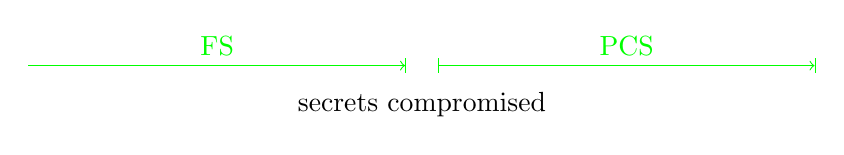
\begin{tikzpicture}%
    \draw [green, ->|] (0,0) -- (4.8,0) node [midway, above] {FS}; %FS arrow
    \node at (5,0) {\color{red}\LARGE\Lightning}; % Corruption
    \node at (5,-.5) {secrets compromised}; 
    \draw [green, |->|] (5.2,0) -- (10,0) node [midway, above] {PCS}; % PCS arrow
\end{tikzpicture}%
    \caption{A sketch of forward and post compromise security.}
    \label{fig:rke:pcs_fs_overview}
\end{figure}

A way to achieve post compromise security are the so-called Ratcheted Key Exchange protocols~(RKE).
In Figure~\ref{fig:rke:overview}, an abstract view on a two party RKE protocol is given.
After the initial key exchange, both parties regularly update their keys in a Ratcheted Key Exchange step.
Using the resulting key, a new message can be encrypted.

For the steps different cryptographic building blocks are used.
For example, X3DH might be used for the initial key exchange, the Signal Double Ratchet algorithm for the Ratcheted Key exchange step and AEAD for the encryption of the messages.

\begin{figure}[!ht]
    \centering
    % !TeX root = ..\..\main.tex
\begin{tikzpicture}
    %draw the cylinder and rotate it so that the "opening" is to the left
    \node[yshift=-2.5cm] (c) at (4.5, 0) [cylinder, shape border rotate=180, draw, minimum height=7cm, minimum width=5cm, anchor=shape center, name path=c1] {};
    
    %first step of ratcheted key exchange 
    \node[yshift=-.5cm] (1) at (c.north) {1. Initial Key Exchange};
    %draw both key derivations
    \node[yshift=-.5cm, xshift=-2.5cm] (1a1) at (1) {$\substack{\downarrow\\\scriptstyle k}$};
    \node[yshift=-.5cm, xshift= 2.5cm] (1a2) at (1) {$\substack{\downarrow\\\scriptstyle k}$};
    %connect the two keys with a dashed arrow (the anchors, e.g. 1a1.30, are "border anchors" that use an angle)
    \draw[<->, dashed] (1a1.30) -- (1a2.150);
    
    %second step
    \node[yshift=-1cm] (2) at (1) {2. Ratcheted Key Exchange};
    %draw refreshing of keys
    \node[yshift=-.5cm, xshift=-2.5cm] (2a1) at (2) {$k\circlearrowleft$};
    \node[yshift=-.5cm, xshift= 2.5cm] (2a2) at (2) {$\circlearrowleft k$};

    %third step
    \node[yshift=-1cm] (3) at (2) {3. Secure Channel};
    %first channel cylinder below the third step (anchor is "shape center", since the normal "center" uses the actual height of the 3d cylinder)
    \node[yshift=-.5cm, anchor=shape center] (3Channel1) at (3) [cylinder, shape border rotate=180, draw, minimum height=5.2cm, minimum width=.5cm] {};
    %draw refreshing keys
    \node[yshift=-1cm, xshift=-2.5cm] (3a1) at (3) {$k\circlearrowleft$};
    \node[yshift=-1cm, xshift= 2.5cm] (3a2) at (3) {$\circlearrowleft k$};
    %second channel cylinder (no anchor=shape center since we use the shape center anchor of the first cylinder for placement)
    \node[yshift=-1cm] (3Channel2) at (3Channel1) [cylinder, shape border rotate=180, draw, minimum height=5.2cm, minimum width=.5cm] {};

    %arrows from the keys in the second step to the first channel in the third step
    \draw [->] (2a1) -- (3Channel1.after top);
    \draw [->] (2a2) -- (3Channel1.before bottom);


    %ALICE and BOB
    \node (A) at (0, 0) {\textbf{Alice}};
    \node (B) at (9, 0) {\textbf{Bob}};

    %the two messages send from Alice
    \node (A_m1) at (0, -3) {$m$};
    \node (A_m2) at (0, -4) {$m$};

    %draw the arrow connecting the first message and the first channel
    %this path is used to get the intersection
    \path[name path=A_m1path] (A_m1) -- (3Channel1.top);
    %calculate the intersections (they are named A_m1_intersect-1, A_m1_intersect-2, ...) and draw the black part of the arrow
    \draw[-,name intersections={of=c1 and A_m1path, name=A_m1_intersect}] (A_m1) -- (A_m1_intersect-1);
    %draw the gray part of the arrow
    \draw[->, gray] (A_m1_intersect-1) -- (3Channel1.top);

    %draw the arrow connecting the second message and the second channel
    \path[name path=A_m2path] (A_m2) -- (3Channel2.top);
    \draw[<-,name intersections={of=c1 and A_m2path, name=A_m2_intersect}] (A_m2) -- (A_m2_intersect-1);
    \draw[-, gray] (A_m2_intersect-1) -- (3Channel2.top);

    %the messages bob receives
    \node (B_m1) at (9, -3) {$m$};
    \node (B_m2) at (9, -4) {$m$};

    %arrows connecting the first channel to bobs first message
    \path[name path=B_m1path] (B_m1) -- (3Channel1.bottom);
    %the gray and black parts of the arrow are switched
    \draw[-,,gray, name intersections={of=c1 and B_m1path, name=B_m1_intersect}] (3Channel1.bottom) -- (B_m1_intersect-1);
    \draw[->] (B_m1_intersect-1) -- (B_m1);

    %arrows connecting the second channel to bobs second message
    \path[name path=B_m2path] (B_m2) -- (3Channel2.top);
    \draw[<-, gray, name intersections={of=c1 and B_m2path, name=B_m2_intersect}] (3Channel2.bottom) -- (B_m2_intersect-1);
    \draw[-] (B_m2_intersect-1) -- (B_m2);

    %Left side FS-arrows
    \draw[->|, green] (.5, -.5) -- (.5, -1.25) node [midway,left] {FS};
    \node at (.5, -1.5) {\color{red}\Large\Lightning}; % corruption arrow
    \draw[|->|, green] (.5, -1.75) -- (.5, -3.25);
    \draw[|->, green] (.5, -3.75) -- (.5, -5);

    %Right side FS-arrows
    \draw[->|, green] (8.5, -.5) -- (8.5, -1.25);
    \draw[|->|, green] (8.5, -1.75) -- (8.5, -3.25);
    \node at (8.5, -3.5) {\color{red}\Large\Lightning}; %corruption arrow
    \draw[|->, green] (8.5, -3.75) -- (8.5, -5) node [midway, right] {PCS};

\end{tikzpicture}
    \caption{Overview of the Ratcheted Key Exchange~(RKE) protocol.
    \alert{PR: would it be possible to align the keys $k$ with their circle arrow horizontally identically? (currently the lower keys are slightly shifted to the right)}}
    \label{fig:rke:overview}
\end{figure}

\paragraph{Types of RKE}
\alert{PR: add history starting with Double Ratchet, then its analysis~\cite{JC:CCDGS20}, then unidirectional~\cite{C:BSJNS17}, then more~\cite{C:PoeRos18}}
RKE protocols can be divided into three types, depending on the directions of communication they support.
Bidirectional RKE protocols is the intuitive case, where full bidirectional communication is supported~(Figure~\ref{fig:RKE:bi}).

Sesquidirectional RKE gives one party full functionality, while the other party can only send ``non-functional'' messages.
Consider for example the ciphertext $c_3$ in Figure~\ref{fig:RKE:sesq}:
It does not encapsulate a key, instead it should be used for efficiency or security (e.g. Bob can use this message to communicate fresh randomness to Alice to recover from earlier compromise).
Every Sesquidirectional RKE protocol can be transformed into a bidirectional RKE protocol, by using two instances of the Sesquidirectional RKE protocol.

\begin{figure}[!ht]
    \centering
    \begin{subfigure}{.5\textwidth}
        \centering
        \input{figures/rke/rke_bi}
        \caption{Bidirectional RKE protocol.}
        \label{fig:RKE:bi}
    \end{subfigure}\hfill
    \begin{subfigure}{.5\textwidth}
        \centering
        % !TeX root = ..\..\main.tex

%%%%%%%%%%%%%
% Arrow are drawn using Tikz overlay and tikzmark, since arrows cross rows in the table.
% tikzmark: https://texdoc.org/serve/tikzmark/0
% using tikzmark requires two compilation passes (this should be fine since we already have to do LaTeX->BibTeX->LaTeX)
%%%%%%%%%%%%%
\begin{tabular}{rC{4cm}l}
    \textbf{Alice} &  & \textbf{Bob} \\
    %save the left and right positions for init arrow using tikzmarks
    %this arrow could also be drawn in the table, but then consistent spacing in relation to the arrows below is hard
    $\st_A$\tikzmark{rke_sesq_init_l} & & \tikzmark{rke_sesq_init_r}$\st_B$ \\
    $\downarrow$ &  & $\downarrow$ \\ 
    $k_1\gets\mathrm{snd}$\tikzmark{rke_sesq_c1_l} &  & \tikzmark{rke_sesq_c1_r}$\mathrm{rcv}\to k_1$ \\
    $\downarrow$ &  & $\downarrow$ \\  
    $k_2\gets\mathrm{snd}$\tikzmark{rke_sesq_c2_l} &  & \tikzmark{rke_sesq_c3_r}$\mathrm{snd}$ \\
    $\downarrow$ &  & $\downarrow$ \\
    $\mathrm{rcv}$\tikzmark{rke_sesq_c3_l} & & \tikzmark{rke_sesq_c2_r}$\mathrm{rcv}\to k_2$ \\
    $\downarrow$ &  & $\downarrow$ \\
\end{tabular}
%draw the arrows
%tikzmark coordinates can be accessed with (pic cs:<name>)
%we shift the coordinates up so that the arrows are roughly in the middle of the line
\begin{tikzpicture}[remember picture,overlay]
    \draw[<->] ([xshift=.2cm, yshift=1mm]pic cs:rke_sesq_init_l) -- ([xshift=-.2cm, yshift=1mm]pic cs:rke_sesq_init_r) node[above, midway] {init};
    \draw[->] ([xshift=.2cm, yshift=1mm]pic cs:rke_sesq_c1_l) -- ([xshift=-.2cm, yshift=1mm]pic cs:rke_sesq_c1_r) node[above, midway] {$c_1$};
    %edge[out=0,in=180,->] curves the arrow
    %the node is placed using xshift, because using the more readable node[midway, near start] causes placement to break
    \draw ([xshift=.2cm, yshift=1mm]pic cs:rke_sesq_c2_l) edge[out=0,in=180,->] ([xshift=-.2cm, yshift=1mm]pic cs:rke_sesq_c2_r) node[above, xshift=.5cm] {$c_2$};
    \draw ([xshift=-.2cm, yshift=1mm]pic cs:rke_sesq_c3_r) edge[out=180,in=0,->] ([xshift=.2cm, yshift=1mm]pic cs:rke_sesq_c3_l) node[above, xshift=-.5cm] {$c_3$};
\end{tikzpicture}
        \caption{Sesquidirectional RKE protocol.}
        \label{fig:RKE:sesq}
    \end{subfigure}
    \caption{Interaction in bi- and sesquidirectional RKE protocols.}
\end{figure}

The third type of RKE protocols is unidirectional RKE, which only allows one party to send.
For simplicity, this is the type of RKE we will focus on in the following.

\subsection{Unidirectional RKE}

An overview of the unidirectional RKE protocol is given in Figure~\ref{fig:rke:uni}.
It should be noted that Bob is purely deterministic.
He can not distribute fresh randomness, and therefore can not recover from corruptions.

\begin{figure}[!ht]
    \centering
    % !TeX root = ..\..\main.tex
\begin{tabular}{rC{4cm}l}
    \textbf{Alice} &  & \textbf{Bob} \\
    $\st_A$ & $\xleftrightarrow{\makebox[3.5cm]{init}}$ & $\st_B$ \\
    $\downarrow$ &  & $\downarrow$ \\ 
    $k_1\gets\mathrm{snd}$ & $\xrightarrow{\mathmakebox[3.5cm]{c_1}}$ & $\mathrm{rcv}\to k_1$ \\
    $\downarrow$ &  & $\downarrow$ \\  
    $k_2\gets\mathrm{snd}$ & $\xrightarrow{\mathmakebox[3.5cm]{c_2}}$ & $\mathrm{rcv}\to k_2$ \\
    $\downarrow$ &  & $\downarrow$ \\
\end{tabular}
    \caption{Unidirectional RKE protocol.}
    \label{fig:rke:uni}
\end{figure}

\paragraph{Syntax} A unidirectional RKE protocol $\URKE=(\URKEinit, \URKEsnd, \URKErcv)$ has the following syntax:

\begin{itemize}
    \item $\URKEinit: \emptyset\tor\stsp_A\times\stsp_B$
    \item $\URKEsnd: \stsp_A\tor\stsp_A\times\ksp\times\csp$
    \item $\URKErcv: \stsp_B\times\csp\to\stsp_B\times\ksp$
\end{itemize}

\paragraph{Correctness} The correctness of $\URKE$ is defined as follows:
\begin{align*} %too long to fit on one line
    \Pr[k_A^i=k_B^i\mid &(\st_A^0, \st_B^0)\getsr\URKEinit, \\
                        &(\st_A^i, k_A^i, c_A^i)\getsr\URKEsnd(\st_A^{i-1}), \\
                        &(\st_B^i, k_B^i)\gets\URKErcv(\st_B^{i-1}, c_B^i)] = 1
\end{align*}

\paragraph{Security} The advantage of an adversary $\advA$ against the $\IND_\URKE^b$ game shown in Figure~\ref{fig:urke:ind} is defined as follows:
\[\Adv_\URKE^\ind(\advA) = \left|\Pr[\IND_\URKE^0(\advA)=1] - \Pr[\IND_\URKE^1(\advA)=1]\right|\]

\begin{figure}[!ht]
    \centering
    \nicoresetlinenr%
    \fbox{%
        \scalebox{\codescalefactor}{%
            %!TEX root=../../main.tex
\markersetlen{ndL}{130pt}%
\markersetlen{ndC}{155pt}%
\markersetlen{ndR}{150pt}%
\newcommand{\sync}{\mathit{sync}}%
\begin{tabular}[t]{lll}
    \nicodemusbox{\markerlenndL}{%
        \textbf{Game} $\IND_{\URKE}^b(\advA)$
        \begin{nicodemus}
            \item $s\gets0; r\gets0; \sync\gets1$
            \item $X_S\gets\emptyset; X_R\gets0$\quad{\color{gray}T3,T4}
            \item $C[\cdot]\gets\bot$
            \item $(\st_A, \st_B)\getsr\URKEinit$
            \item $b'\getsr\advA$
            \item Stop with~$b'$
        \end{nicodemus}%
        \medskip

        \textbf{Oracle} $\Oexps()$
        \begin{nicodemus}
            \item $X_S\gets X_S\cup\{s\}$\quad{\color{gray}T4}
            \item Return~$\st_A$
        \end{nicodemus}
    }%
    &
    \nicodemusbox{\markerlenndC}{%
        \textbf{Oracle} $\Osnd()$
        \begin{nicodemus}
            \item If $X_A=1$: Return~$(\bot, \bot)$\quad{\color{gray}T3}
            \item $(\st_A, k_0, c)\getsr\URKEsnd(\st_A)$
            \item $k_1\getsr\ksp$
            \item $C[s]\gets c$
            \item $s\gets s+1$
            \item Return~$(k_b,c)$
        \end{nicodemus}%
        \medskip

        \textbf{Oracle} $\Oexpr()$
        \begin{nicodemus}
            \item If $\sync=1\land s>r$:\quad{\color{gray}T2}
            \item \quad Return~$\bot$
            \item If $\sync=1\land s=r$:\quad{\color{gray}T3}
            \item \quad $X_R\gets1$
            \item Return~$\st_B$
        \end{nicodemus}
    }%
    &
    \nicodemusbox{\markerlenndR}{%
        \textbf{Oracle} $\Orcv(c)$
        \begin{nicodemus}
            \item $(\st_B, k_0)\gets\URKErcv(\st_B, c)$
            \item If $c\neq C[r] \land \sync=1$:
            \item \quad $\sync\gets0$
            \item \quad If $r\not\in X_S\land k_0\neq\bot$:\quad{\color{gray}T4}
            \item \qquad $k_1\getsr\ksp$
            \item \qquad Return~$k_b$
            \item $r\gets r+1$
            \item If $\sync=1$:\quad{\color{gray}T1}
            \item \quad Return~$\bot$
            \item Stop with~$b'$
        \end{nicodemus}%
    }%
\end{tabular}%%
        }%
    }
    \caption{%
        Games $\IND$ for unidirectional RKE~$\URKE$. Lines accounting for trivial attacks T1-T4 are marked.
    }
    \label{fig:urke:ind}
\end{figure}

\paragraph{Trivial winning conditions} The four trivial attacks against the game $\IND_\URKE^b$ are shown in Figure~\ref{fig:urke:trivial}.

\begin{figure}[!ht]
    \centering
    \begin{minipage}[t]{.5\textwidth}
        Attack 1: Challenge on both Sides:
        \begin{enumerate}[topsep=\smallskipamount]
            \item $\Osnd()\to(k,c)$
            \item $\Orcv(c)\to(k')$
            \item Stop with $(k\neq k')$
        \end{enumerate}
        \medskip
        Attack 2: Send + Receiver Exposure:
        \begin{enumerate}[topsep=\smallskipamount]
            \item $\Osnd()\to(k,c)$
            \item $\Oexpr()\to\st_R$
            \item $(st_R', k')\gets\URKErcv(st_R, c)$
            \item Stop with $(k\neq k')$
        \end{enumerate}
    \end{minipage}\hfill%
    \begin{minipage}[t]{.5\textwidth}
        Attack 3: Receiver Exposure + Send:
        \begin{enumerate}[topsep=\smallskipamount]
            \item $\Oexpr()\to\st_R$
            \item $\Osnd()\to(k,c)$
            \item $(st_R', k')\gets\URKErcv(st_R, c)$
            \item Stop with $(k\neq k')$
        \end{enumerate}
        \medskip
        Attack 4: Sender Impersonation:
        \begin{enumerate}[topsep=\smallskipamount]
            \item $\Oexps()\to\st_S$
            \item $(st_S', k', c')\getsr\URKEsnd(st_S)$
            \item $\Orcv(c')\to(k)$
            \item Stop with $(k\neq k')$
        \end{enumerate}
    \end{minipage}
    \caption{Trivial winning conditions for game $\IND_\URKE^b$.}
    \label{fig:urke:trivial}
\end{figure}

%this paragraph is not precise and understandable enough in my opinion
\paragraph{Intuitive Security Goals} The security goal for unidirectional RKE protocols is to ensure that sender and receiver exposures are as harmless as possible.
In particular, the sender state should only allow for \emph{immediate} impersonations, i.e. it should not reveal any (challenge) keys except the one received in the impersonation.
The receiver state should only reveal future ``compatible'' (challenge) keys; an active attacker breaks ``compatibility''.

This means that the protocol is forward secure w.r.t. exposures of senders and receivers.
Post-compromise security is only achieved for the sender, who is also hard to non-trivially impersonate.


\paragraph{Construction} A construction for a unidirectional RKE protocol $\URKE$ is given in Figure~\ref{fig:urke:const}.

\begin{figure}[!ht]
    \centering
    \nicoresetlinenr%
    \fbox{%
        \scalebox{\codescalefactor}{%
            % !TeX root = ..\..\main.tex
\markersetlen{ndL}{110pt}%
\markersetlen{ndM}{125pt}%
\markersetlen{ndR}{135pt}%
\begin{tabular}[t]{lll}
    \nicodemusbox{\markerlenndL}{%
        \textbf{Proc} $\URKEinit$
        \begin{nicodemus}
            \item $(\dk,\ek)\getsr\KEMgen$
            \item $(\sk,\vk)\getsr\SIGgen$
            \item $t\gets\epsilon$
            \item $\st_S\gets(\ek,\sk,t)$
            \item $\st_R\gets(\ek,\vk,t)$
            \item Return $(\st_S,\st_R)$
        \end{nicodemus}%
    }%
    &
    \nicodemusbox{\markerlenndM}{%
        \textbf{Proc} $\URKEsnd(\st_S)$
        \begin{nicodemus}
            \item $(\ek,\sk,t)\gets\st_S$
            \item $(k', c')\getsr\KEMenc(\ek)$
            \item $(\sk',\vk')\getsr\SIGgen$
            \item $\sigma\getsr\SIGsig(\sk, (c',\vk'))$
            \item $c\gets(c',\vk',\sigma)$
            \item $(k,t,\dk)\gets \ROh(t, k', c)$
            \item $\ek\gets\KEMgen(\dk)$
            \item $\st_S\gets(\ek,\sk',t)$
            \item Return $(\st_S, k, c)$
        \end{nicodemus}%
    }%
    &
    \nicodemusbox{\markerlenndR}{%
        \textbf{Proc} $\URKErcv(\st_R, c)$
        \begin{nicodemus}
            \item $(\dk, \vk, t)\gets\st_R$
            \item $(c', \vk', \sigma)\gets c$
            \item If $\SIGvfy(\vk, (c', \vk'), \sigma) = 0$:
            \item \quad Return $(\bot, \bot)$
            \item $k'\gets\KEMdec(\dk, c')$
            \item $(k,t,\dk)\gets \ROh(t, k', c)$
            \item $\st_R\gets(\dk, \vk', t)$
            \item Return $(\st_R, k)$
        \end{nicodemus}%
    }%
\end{tabular}%%
        }%
    }
    \caption{%
        Construction of $\URKE$ using key encapsulation mechanism $\KEM$, signature $\SIG$ and random oracle $\ROh$.
    }
    \label{fig:urke:const}
\end{figure}

\subsection{Random Oracle Model}

To analyze the security of the unidirectional RKE protocol $\URKE$, we use the random oracle model~(ROM).
The random oracle model is a common abstraction in cryptography and models an ideal hash or one-way function.

In the ``arrows-and-boxes'' style, the random oracle is shown in its own box instead of being called with $h\getsr \ROh$ (see Figure~\ref{fig:rom:overview}).
Reduction and adversary interact with the random oracle just like they normally would.
It is important to keep in mind, that the random oracle is still part of the reduction.


%aligning the minipages with \begin{minipage}[b] might look better
\begin{figure}[!ht]
    \begin{minipage}[]{.5\textwidth}
        \centering
        \nicoresetlinenr%
        \fbox{%
            \scalebox{\codescalefactor}{%
                % !TeX root = ../../main.tex
\markersetlen{ndL}{80pt}%
\newcommand{\CC}{\mathit{CC}}%
\nicodemusbox{\markerlenndL}{%
    \textbf{Oracle} $H(x)$
    \begin{nicodemus}
        \item If $h[x]=\bot:$
        \item \quad$y\getsr\{0,1\}^l$
        \item \quad$h[x]\gets y$
        \item Return~$h[x]$
    \end{nicodemus}%
}%%
            }%
        }
        \caption{%
            Simulation of a random oracle $H$.
        }
        \label{fig:rom:sim}
    \end{minipage}\hfill
    \begin{minipage}[]{.5\textwidth}
        \centering
        % !TeX root = ..\..\main.tex
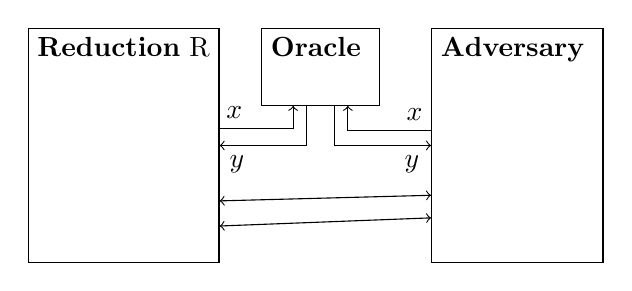
\begin{tikzpicture}
    %draw boxes for reduction oracle and adversary
    %align=left sets the alignment of the text
    %text depth virtually sets the height of the text and therefore shifts the text to the top
    \node[rectangle, draw, minimum width=2cm, align=left, text depth=2.5cm] (R) at (0,0) {\textbf{Reduction} R};
    \node[rectangle, draw, minimum width=1.5cm, align=left, text depth=.5cm] (H) at (2.5,1) {\textbf{Oracle} $\ROh$};
    \node[rectangle, draw, minimum width=2cm, align=left, text depth=2.5cm] (A) at (5,0) {\textbf{Adversary} $\advA$};

    %draw arrows between R and H
    %(R.10) is a border anchor (in angles, i.e. R.0 is at the top center, R.180 at the bottom center)
    %place node above the arrow. pos sets the position from beginning (pos=0) to end (pos=1)
    %using -| instead of -- makes the arrow bend
    \draw[->] (R.10) -| (H.235) node[pos=.1, above] {$x$};
    \draw[<-] (R.0) -| (H.250) node[pos=.1, below] {$y$};

    %draw arrows between H and A
    \draw[->] (A.170) -| (H.305) node[pos=.1, above] {$x$};
    \draw[<-] (A.180) -| (H.290) node[pos=.1, below] {$y$};

    %draw arrows between R and A
    \draw[<->] (R.330) -- (A.210);
    \draw[<->] (R.320) -- (A.220);
\end{tikzpicture}
        \caption{%
            Interaction with random oracle $H$ in the ``arrows-and-boxes'' style.
        }
        \label{fig:rom:overview}
    \end{minipage}
\end{figure}

\subsection{Security Proof of URKE in the ROM}

\paragraph{Proof Sketch} 
First, assume that the verification key $\vk_i$ is authentically transmitted based on authenticity of signature $\sig_{i-1}$.
This implies that the ciphertext $c_i$ is transmitted authentically unless the sender is trivially impersonated.
The first assumption can be reduced to the $\SUFCMA$ security of the underlying signature scheme $\SIG$.

Secondly, assume that the ciphertext $c_i$ protects the intermediate key $k'$.
Then the random oracle input in the $i$-th send operation is secret, which implies that the random oracle output is also secret.
We can then assume, that the $i+1$-th $\KEM$ instance protects the $i+1$-th ciphertext and its key, which can be reduced to the $\INDCCA$ security of the $\KEM$.

\paragraph{Theorem}
The proof sketch gives a preliminary security bound:

For every successful adversary $\advA$ against $\IND$ security of scheme $\URKE$, there exist adversaries $\advB_\SIG$ and $\advB_\KEM$ such that
\[\Adv_\URKE^\ind (\advA)\leq x\cdot \Adv_\SIG^\sufcma(\advB_\SIG) + y\cdot \Adv_\KEM^\indcca(\advB_\KEM)+z\]

The need for the factors $x, y$ and $z$ becomes clear in the concrete proof in the next section.

\paragraph{Formal Proof}
We now prove the security of the $\URKE$ scheme through a series of games:

%set game i as the itemize bullet points to ensure no text under the game i label
\begin{itemize}[leftmargin=2.0cm]
    \item[Game 0:] The original game $\IND_\URKE^b$.
    \item[Game 1:] Guess $n_{forge}\getsr [q_{rcv}+1]$, where $q_{rcv}$ is the number of queries to $\Orcv$.
        If the $n_{forge}$-th query to oracle $\Orcv$ is not one that flips the bit $\mathit{sync}$ from $1$ to $0$, abort the game.

        It holds that $\Adv^0=\Adv^1\cdot(q_{rcv}+1)$.
    \item[Game 2:] If in the $n_{forge}$-th query to oracle $\Orcv$ the sender was not exposed for the corresponding prior state (i.e.,$n_{forge}\notin X_S$) and the received ciphertext was accepted (i.e., $k_0\neq\bot$), then abort the game.
        The advantage is
        \[\Adv^1\leq\Adv^2 + \Adv_{\SIG}^\sufcma(\advB_\SIG)\]
    \item[Game 3:] Guess $n_{exp}\getsr [q_{rcv}]$.
        If the receiver state is not exposed for the first time after the $n_{exp}$-th query to oracle $\Orcv$, abort the game.

        It holds that $\Adv^2=\Adv^3\cdot q_{rcv}$.
        
    \listintertext{For the next games we use the hybrid argument over $n_{snd}$ steps, where $n_{snd}=\begin{cases}
        q_{snd} &, n_{exp}>n_{forge}\\
        n_{exp} &, \text{otherwise}
    \end{cases}$}
    \item[Game 4:] Lazy sample output of random oracle in the $i$-th query to $\Osnd$.
        Lazy sampling means, that the output of the random oracle gets computed only when the adversary queries the corresponding inputs ``externally''. 

        It is $\Adv^3=\Adv^4$.
    \item[Game 5:] Abort if the adversary queries the random oracle for the inputs specified by the $i$-th query to oracle $\Osnd$.
        The advantage is
        \[\Adv^4\leq\Adv^5 + \Adv_\KEM^\owcca(\advB_\KEM)\]
\end{itemize}

We show indistinguishability of game 1 and game 2 by reducing every successful distinguisher $\advD_1^2$ to a successful attacker against the $\SUFCMA$ security (Figure~\ref{fig:sig:suf}) of the signature scheme $\SIG$.

\begin{itemize}
    \item Simulation
    \begin{itemize}
        \item Oracle $\Osnd$: 
        In $n_{forge}-1$-th query embed the verification key $\vk$ in $c$.\par
        In $n_{forge}$-th query ask the signing oracle of $\SUFCMA$ game for $\sig$ with $m:=(c',\vk')$.
        \item  Oracle $\Oexpr$: 
        After $n_{forge}-1$-th query to $\Orcv$, embed $\vk$ in $\st_R$.
        \item Everything else is simulated honestly
    \end{itemize}
    \item Extraction: Distinguisher $\advD_1^2$ can only distinguish between game 1 and game 2 if game 2 aborts.
    This only happens upon successful signature forgery.
\end{itemize}

Similarly, we prove indistinguishability of games 4 and 5 for every distinguisher $\advD_4^5$ by reducing to $\OWCCA$ security (Figure~\ref{fig:kem:ow:cca}) of the $\KEM$.

\begin{itemize}
    \item Simulation
    \begin{itemize}
        \item Oracle $\Oexps$: 
        After the $i-1$-th query to $\Osnd$, embed the encapsulation key $\ek$ in $\sk_S$.
        \item  Oracle $\Osnd$: 
        In $i$-th query, embed the challenge ciphertext $c^*$ from the underlying $OWCCA_\KEM$ game as the $\KEM$ ciphertext 
        \item Oracle $\Orcv(c)$: If $c$ was a trivial impersonation in $i$-th query to $\Orcv$, use oracle $\Odec$ of $\OWCCA$ game.
    \end{itemize}
    \item Extraction: The only way to distinguish games 4 and 5 for the adversary is to query the random oracle with the same inputs as the $i$-th $\Osnd$ query would.
    Then, if the random oracle is queried with $x=(t,k',c)$ s.t. $t$ and $c$ match with internal values for $i$-th $\Osnd$ query, send $k'$ to $\OWCCA$ game.

\end{itemize}

After the $n_{snd}$-th hybrid step in game 5, all challenge keys are random oracle outputs for which adversary $\advA$ never queried random oracle on the corresponding inputs.
It follows that $\Adv^5=0$.

Taking the advantages together, the following concrete security bound for scheme $\URKE$ can be formulated:
\[\Adv_\URKE^\ind(\advA) \leq (q_{rcv}+1)\cdot(\Adv_\SIG^\sufcma(\advB_\SIG)+q_{rcv}\cdot q_{snd}\Adv_\KEM^\owcca(\advB_\KEM))\] 


%ALTERNATIVE: both proofs (indistinguishability of games 1 and 2 and games 4 and 5) as in the lecture (simulation written in boxes-and-arrows style):
% \begin{figure}[!ht]
%     \centering
%     %!TEX root=../../main.tex
\newcommand{\MS}{\mathit{MS}}%
\begin{tabular}{lllll}
    \algbox{4cm}{%
        \textbf{Game} $\SUFCMA_\SIG$:\\
        $\MS\gets\emptyset$\\
        $(\sk,\vk)\getsr\SIGgen$\\
        \\
        $\sig\gets\SIGsig(\sk, m)$\\
        $\MS\gets\MS\cup\{(m, \sig)\}$\\
        \\
        If $\SIGvfy(\vk, m^*, \sig^*)=1$:\\
        $\land (m^*,\sig^*)$:\\
        \hspace*{1em}Stop with~$1$\\ %\quad does not work; but quad should have length 1em
        Stop with~$0$}&
    \arrbox{1cm}{%
        $\xrightarrow{\vk}$\\~\\  
        $\xleftarrow{m}$\\
        $\xrightarrow{\sig}$\\~\\
        $\xleftarrow{m^*,\sig^*}$}&
    \algbox{6.5cm}{%
        \textbf{Reduction} $\mathcal{R}$
        \begin{itemize}
            \item Oracle $\Osnd$: 
            In $n_{forge}-1$-th query embed the verification key $\vk$ in $c$.\par
            In $n_{forge}$-th query ask the signing oracle of $\SUFCMA$ game for $\sig$ with $m:=(c',\vk')$.
            \item  Oracle $\Oexpr$: 
            After $n_{forge}-1$-th query to $\Orcv$, embed $\vk$ in $\st_R$.
            \item Everything else is simulated honestly
        \end{itemize}
    }&
    \arrbox{1cm}{
        $\leftrightarrow$\\~\\~\\~\\
        $\xleftarrow{d}$}&
    \algbox{2.5cm}{%
        \textbf{Adversary} $\advD_1^2$\\~\\~\\~\\~\\~\\~\\~\\}
\end{tabular}
%     \caption{Indistinguishability of games 1 and 2 for distinguisher $\advD_1^2$.}
%     \label{fig:urke:ind:games1_2}
% \end{figure}

% \begin{figure}[!ht]
%     \centering
%     %!TEX root=../../main.tex
\newcommand{\CC}{\mathit{CC}}%
\begin{tabular}{lllll}
    \algbox{4cm}{%
        \textbf{Game} $\\OWCCA_\KEM$:\\
        $(\dk,\ek)\getsr\KEMgen$\\~\\
        $(k^*, c^*)\getsr\KEMenc(\ek)$\\~\\
        If $c\neq c^*:$\\
        \hspace*{1em}$k\gets\KEMdec(\dk, c)$\\
        If $k'\neq k^*$:\\
        \hspace*{1em}$\mathit{no}\gets1$\\
        Else: Stop with~$1$\\
        Stop with~$0$}&
    \arrbox{1cm}{%
        $\xrightarrow{\ek}$\\~\\  
        $\xrightarrow{c^*}$\\~\\
        $\xleftarrow{c}$\\
        $\xrightarrow{k}$\\
        $\xleftarrow{k'}$\\
        $\xrightarrow{\mathit{no}}$}&
    \algbox{6.5cm}{%
        \textbf{Reduction} $\mathcal{R}$
        \begin{itemize}
            \item Oracle $\Oexps$: 
            After the $i-1$-th query to $\Osnd$, embed the encapsulation key $\ek$ in $\sk_S$.
            \item  Oracle $\Osnd$: 
            In $i$-th query, embed the challenge ciphertext $c^*$ from the underlying $OWCCA_\KEM$ game as the $\KEM$ ciphertext 
            \item Oracle $\Orcv(c)$: If $c$ was a trivial impersonation in $i$-th query to $\Orcv$, use oracle $\Odec$ of $\OWCCA$ game.
        \end{itemize}
    }&
    \arrbox{1cm}{
        $\leftrightarrow$\\~\\~\\~\\
        $\xleftarrow{d}$}&
    \algbox{2.5cm}{%
        \textbf{Adversary} $\advD_4^5$\\~\\~\\~\\~\\~\\~\\~\\~\\~\\~\\}
\end{tabular}
%     \caption{Indistinguishability of games 4 and 5 for distinguisher $\advD_4^5$.}
%     \label{fig:urke:ind:games4_5}
% \end{figure}